\documentclass[UTF8]{ctexart}

\usepackage{mathpazo,euler}
\usepackage[T1]{fontenc}
\usepackage{dejavu}

\usepackage{xcolor}

\definecolor{dkgreen}{rgb}{0,0.6,0}
\definecolor{gray}{rgb}{0.5,0.5,0.5}
\definecolor{mauve}{rgb}{0.58,0,0.82}

\usepackage{graphicx}

\usepackage{tikz}

\usepackage{listings}

\lstset{ %
  language=R,                     % the language of the code
  basicstyle=\scriptsize,         % the size of the fonts that are used for the code
  % numbers=left,                   % where to put the line-numbers
  % numberstyle=\tiny\color{gray},  % the style that is used for the line-numbers
  % stepnumber=1,                   % the step between two line-numbers. If it's 1, each line
                                  % will be numbered
  % numbersep=5pt,                  % how far the line-numbers are from the code
  % backgroundcolor=\color{white},  % choose the background color. You must add \usepackage{color}
  showspaces=false,               % show spaces adding particular underscores
  showstringspaces=false,         % underline spaces within strings
  showtabs=false,                 % show tabs within strings adding particular underscores
  % frame=single,                   % adds a frame around the code
  rulecolor=\color{black},        % if not set, the frame-color may be changed on line-breaks within not-black text (e.g. commens (green here))
  tabsize=2,                      % sets default tabsize to 2 spaces
  captionpos=b,                   % sets the caption-position to bottom
  breaklines=true,                % sets automatic line breaking
  breakatwhitespace=false,        % sets if automatic breaks should only happen at whitespace
  title=\lstname,                 % show the filename of files included with \lstinputlisting;
                                  % also try caption instead of title
  keywordstyle=\color{blue},      % keyword style
  commentstyle=\color{dkgreen},   % comment style
  stringstyle=\color{mauve},      % string literal style
  escapeinside={\%*}{*)},         % if you want to add a comment within your code
  morekeywords={*,...}            % if you want to add more keywords to the set
}

\begin{document}

\begin{titlepage}

\tikz[remember picture,overlay] \node[opacity=0.3,inner sep=0pt] at (current page.center){
\includegraphics[width=\paperwidth,height=\paperheight]{cover.pdf}};
% \clearpage


  \centering
  
	{\scshape\Huge 现代统计图形 \par}
  {\scshape\huge Modern Statistical Graphics\par}
  \vspace*{\baselineskip}
	\vfill
	{\LARGE\itshape 
	谢益辉\\
	黄湘云\\
  赵鹏
\par
}
\vspace*{\baselineskip}
\vfill

\begin{lstlisting}
par(mar = c(0.2, 0.2, 0.2, 0.2), mfrow = c(2, 2))
for (n in c(63, 60, 76, 74)) {
  set.seed(711)
  plot.new()
  box()
  size <- c(replicate(n, 1 / rbeta(2, 1.5, 4)))
  center <- t(replicate(n, runif(2)))[rep(1:n, each = 2), ]
  color <- paste("#", apply(
    replicate(2 * n, sample(c(0:9, LETTERS[1:6]), 8, TRUE)), 2, paste,
    collapse = ""
  ), sep = "")
  points(center, cex = size, pch = rep(20:21, n), col = color)
}
\end{lstlisting}
\vspace*{\baselineskip}
\vfill

% Bottom of the page
  {\large \today\par}
  \vspace*{\baselineskip}
\vfill
  \raggedleft
  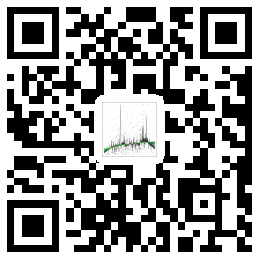
\includegraphics[width=0.25\textwidth]{QR-code.png}

\end{titlepage}
 
\end{document}
